\chapter{Tijd meten}\label{ch:g2:measuring-time}

``Nog vijf minuutjes!'' --- maar hoe lang is dat eigenlijk? Tijd kun je
niet zien, niet vasthouden en niet langs een liniaal leggen. En toch
\omterm{def:g2:measuring-length:measure}{meten} we hem elke dag: wedstrijden hebben winnaars, taarten komen
niet rauw en niet verbrand uit de oven, en de school stopt op het
juiste moment. Laten we leren hoe de tijd getemd wordt.

\section{Tijdstippen en tijdsduren}

\begin{example}[De volgorde van de dag]\label{ex:g2:measuring-time:order}
Een dag is een optocht van gebeurtenissen, altijd op volgorde: opstaan,
ontbijt, school, lunch, middag, avondeten, bed. ``Het ontbijt komt
\emph{vóór} school'' en ``het avondeten komt \emph{na} de lunch'' ---
vóór en na zijn de eerste woorden van de tijd, net zoals langer en
korter de eerste woorden van de lengte waren.
\end{example}

\begin{omfigure}
\begin{tikzpicture}[scale=0.85]
  \draw[-Stealth, very thick] (0,0) -- (11.4,0);
  \foreach \x/\name in {0.8/opstaan, 2.9/ontbijt, 5.0/school,
      7.1/lunch, 9.2/avondeten, 10.7/bed} {
    \fill[omDef] (\x,0) circle (2.4pt);
    \node[above, font=\small, rotate=40, anchor=south west]
      at (\x,0.15) {\name};
  }
\end{tikzpicture}

{\small Eén dag uitgezet als een getallenlijn: elke gebeurtenis heeft
haar plaats, en de pijl laat zien welke kant de tijd op stroomt ---
altijd vooruit.}
\end{omfigure}

\begin{definition}[Tijdsduur]\label{def:g2:measuring-time:duration}
Een \emph{tijdstip}\index{tijdstip} is één punt van de dag: het moment
waarop de bel gaat. Een \emph{tijdsduur}\index{tijdsduur} is het stuk
tijd tussen twee tijdstippen: van de bel tot het einde van de les.
Tijdstippen beantwoorden \emph{wanneer?}; tijdsduren beantwoorden
\emph{hoe lang?}
\end{definition}

\begin{example}[Wanneer of hoe lang?]\label{ex:g2:measuring-time:whenhowlong}
``De film begint na het avondeten'' gaat over een \omterm{def:g2:measuring-time:duration}{tijdstip}. ``De film
duurt zo lang als twee middagpauzes'' gaat over een \omterm{def:g2:measuring-time:duration}{tijdsduur}. ``Mijn
verjaardag is in de lente'': \omterm{def:g2:measuring-time:duration}{tijdstip}. ``De vakantie voelde zo kort'':
\omterm{def:g2:measuring-time:duration}{tijdsduur} --- en dit hoofdstuk gaat vooral over tijdsduren.
\end{example}

\section{Tijdsduren vergelijken}

\begin{method}[Een eerlijke wedstrijd tussen tijdsduren]\label{met:g2:measuring-time:race}
Om te vinden welke van twee dingen langer duurt:
\begin{enumerate}
  \item start ze allebei op \emph{hetzelfde \omterm{def:g2:measuring-time:duration}{tijdstip}} --- ``klaar voor
        de start, af!'';
  \item kijk welke het eerst klaar is;
  \item degene die nog bezig is als de ander klaar is, duurt langer.
\end{enumerate}
Kunnen ze niet samen lopen (het bad van vandaag en het avondeten van
gisteren), laat ze dan allebei racen tegen \emph{hetzelfde} derde
ding --- een zandloper.
\end{method}

\begin{example}[De zandloper]\label{ex:g2:measuring-time:sandtimer}
Een zandloper is een glaasje met een smalle taille: het zand doet er
altijd \emph{dezelfde} \omterm{def:g2:measuring-time:duration}{tijdsduur} over om door te lopen. Daarmee is hij
een scheidsrechter. Tandenpoetsen tegen de zandloper: het zand was
eerder op --- langer poetsen! Een liedje tegen de zandloper: het
liedje won. Het liedje duurt dus langer dan het tandenpoetsen, ook al
hebben ze nooit rechtstreeks tegen elkaar geracet.
\end{example}

\begin{omfigure}
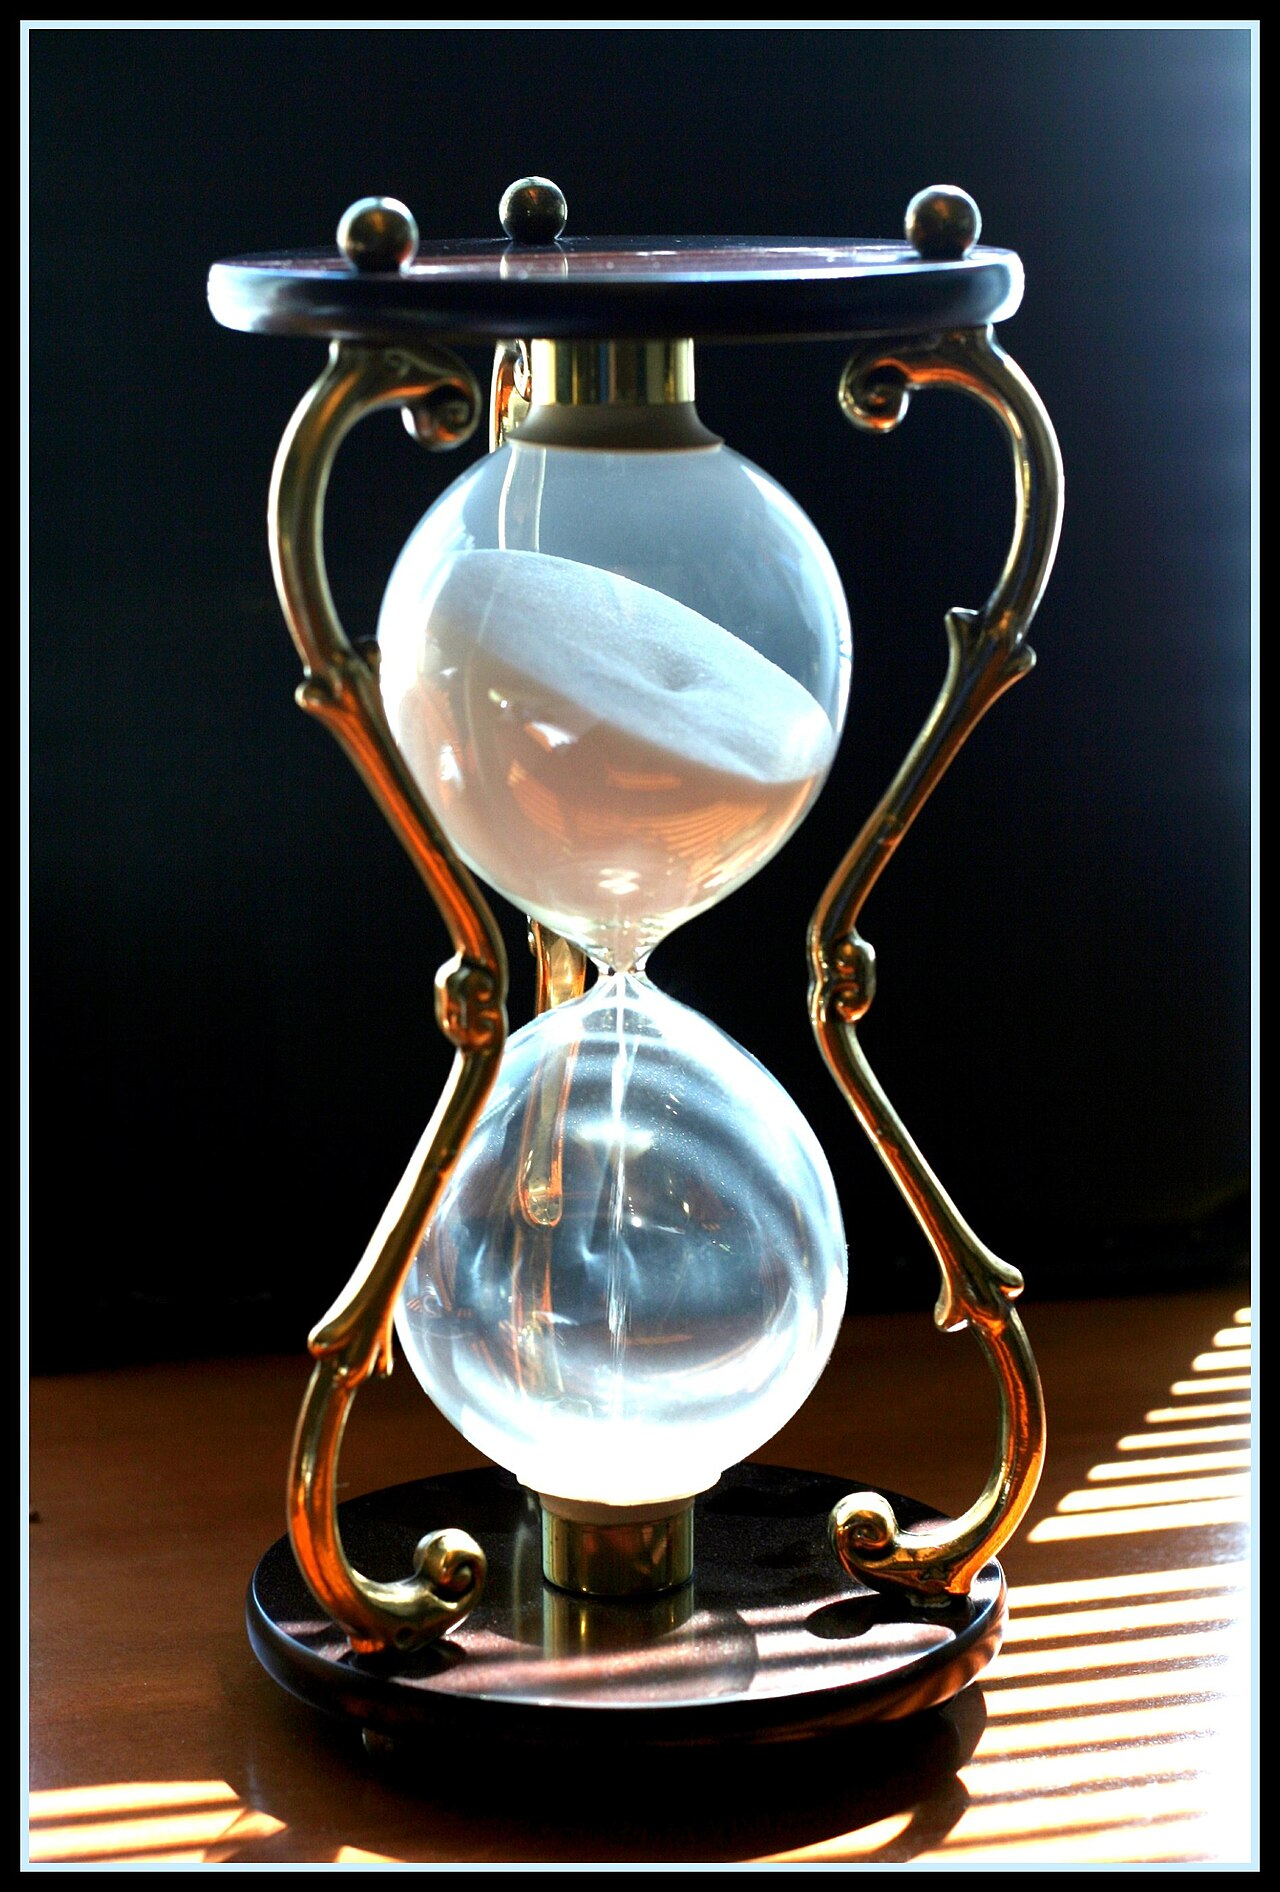
\includegraphics[width=0.34\linewidth]{images/book1/hourglass.jpg}

{\small Een zandloper: een \omterm{def:g2:measuring-time:duration}{tijdsduur} die je in je hand kunt houden. Het
zand heeft altijd evenveel tijd nodig om door de smalle taille te
glippen --- draai hem om, en hij fluit weer. \emph{Foto: John Morgan,
CC BY 2.0.}}
\end{omfigure}

\begin{remark}[Gevoelens zijn slechte klokken]\label{rem:g2:measuring-time:feelings}
Een leuke middag vliegt voorbij; een saaie rij kruipt --- en toch kan
de klok voor allebei hetzelfde tellen. Ons tijdsgevoel laat zich
makkelijk bedriegen, net zoals het gevoel zich liet bedriegen over
warm en koud. Juist daarom zijn scheidsrechters als de zandloper
belangrijk: zand verveelt zich niet.
\end{remark}

\section{Gelijkmatige tikken tellen}

\begin{definition}[De seconde]\label{def:g2:measuring-time:second}
De \emph{seconde}\index{seconde} is de \omterm{def:g2:measuring-length:measure}{eenheid} van tijd die over de
hele wereld wordt gebruikt, geschreven \unit{s}. Eén seconde duurt
ongeveer zo lang als één rustige hartslag, of als de gelijkmatige tik
van een grote klok. ``Eenentwintig, tweeëntwintig'' in een rustig
tempo zeggen telt ongeveer één seconde per getal.
\end{definition}

\begin{example}[Probeer het: hoeveel seconden?]\label{ex:g2:measuring-time:count}
Tel gelijkmatig de \omterm{def:g2:measuring-time:second}{seconden} terwijl: je rustig je adem inhoudt; de
kraan een glas vult; een vriend naar het hek rent en terug. Het glas
doet er misschien $6$ \omterm{def:g2:measuring-time:second}{seconden} over, het rennen $20$. Nu kunnen het
tandenpoetsen en het liedje van daarnet \emph{getallen} krijgen ---
en getallen kunnen, net als bij lengtes, reizen en nagekeken worden.
\end{example}

\begin{example}[Uren op de klok]\label{ex:g2:measuring-time:clock}
\omterm{def:g2:measuring-time:second}{Seconden} zijn voor korte dingen. Lange stukken tel je in
\emph{uren}\index{uur}: een schoolochtend duurt \omterm{ex:g2:measuring-time:clock}{uren}, een nacht slaap
ook. De kleine wijzer van de klok wijst het uur aan: recht op de $3$
is het drie uur; tussen $3$ en $4$ met de grote wijzer recht omlaag is
het half vier. Een hele dag en nacht samen tellen $24$ uur ---
terwijl de Aarde, weet je nog, één hele omwenteling maakt.
\end{example}

\begin{omfigure}
\begin{tikzpicture}[scale=0.85]
  \draw[thick] (0,0) circle (1.5);
  \foreach \h in {1,...,12} {
    \node[font=\footnotesize] at ({90-\h*30}:1.22) {\h};
  }
  \draw[very thick, omDef] (0,0) -- ({90-3*30}:0.8);
  \draw[thick, omThm] (0,0) -- (90:1.05);
  \node[below, font=\small] at (0,-1.75) {drie uur};
  \begin{scope}[xshift=6cm]
    \draw[thick] (0,0) circle (1.5);
    \foreach \h in {1,...,12} {
      \node[font=\footnotesize] at ({90-\h*30}:1.22) {\h};
    }
    \draw[very thick, omDef] (0,0) -- ({90-3.5*30}:0.8);
    \draw[thick, omThm] (0,0) -- (270:1.05);
    \node[below, font=\small] at (0,-1.75) {half vier};
  \end{scope}
\end{tikzpicture}

{\small Twee klokken: de kleine wijzer vertelt het uur. Om half vier
is hij halverwege van de $3$ naar de $4$ gelopen.}
\end{omfigure}

\section{Oefeningen}

\begin{exercise}[$\star$]\label{exo:g2:measuring-time:1}
Zet op volgorde: avondeten; \ opstaan; \ buitenspelen in de middag; \
ontbijt; \ bed.
\end{exercise}

\begin{exercise}[$\star$]\label{exo:g2:measuring-time:2}
\omterm{def:g2:measuring-time:duration}{Tijdstip} of \omterm{def:g2:measuring-time:duration}{tijdsduur}? ``De bel gaat om twaalf uur''; \ ``de taart
bakt een half uur''; \ ``we vertrokken na de lunch''; \ ``de reis
voelde eindeloos''.
\end{exercise}

\begin{exercise}[$\star$]\label{exo:g2:measuring-time:3}
Twee kaarsen worden op hetzelfde \omterm{def:g2:measuring-time:duration}{tijdstip} aangestoken; de rode gaat
uit terwijl de blauwe nog brandt. Welke kaars duurde langer? Welke
regel uit \cref{met:g2:measuring-time:race} volgden de kaarsen?
\end{exercise}

\begin{exercise}[$\star$]\label{exo:g2:measuring-time:4}
Waarom is een zandloper een eerlijke scheidsrechter voor
tijdsduren? Wat is er elke keer dat hij wordt omgedraaid altijd
hetzelfde aan hem?
\end{exercise}

\begin{exercise}[$\star$]\label{exo:g2:measuring-time:5}
Ben zegt dat zijn saaie wachttijd bij de tandarts ``een eeuwigheid''
duurde. Zijn horloge zegt dat hij korter duurde dan zijn
lievelingstekenfilm. Hoe kan dat? (Zie
\cref{rem:g2:measuring-time:feelings}.)
\end{exercise}

\begin{exercise}[$\star$]\label{exo:g2:measuring-time:6}
Tel gelijkmatig de \omterm{def:g2:measuring-time:second}{seconden} en meet: hoeveel \omterm{def:g2:measuring-time:second}{seconden} heb je nodig om
je volledige naam te schrijven? Om je schoenen aan te trekken?
\end{exercise}

\begin{exercise}[$\star$]\label{exo:g2:measuring-time:7}
Welke \omterm{def:g2:measuring-length:measure}{eenheid} past beter, \omterm{def:g2:measuring-time:second}{seconden} of \omterm{ex:g2:measuring-time:clock}{uren}: een niesbui; \ een
nacht slaap; \ een veter strikken; \ een schoolochtend?
\end{exercise}

\begin{exercise}[$\star$]\label{exo:g2:measuring-time:8}
Teken een klok die vijf uur aanwijst, en een andere die half zes
aanwijst. Waar wijst de kleine wijzer om half zes naartoe?
\end{exercise}

\begin{exercise}[$\star\star$]\label{exo:g2:measuring-time:9}
Het bad van gisteren en de douche van vandaag kunnen niet tegen elkaar
racen. Leg stap voor stap uit hoe je met één zandloper uitzoekt welke
langer duurt --- en wat je opschrijft zodat je vriend het kan
nakijken.
\end{exercise}

\begin{exercise}[$\star\star$]\label{exo:g2:measuring-time:10}
Lila telt ``een, twee, drie\dots'' heel snel en zegt dat het glas in
$12$ \omterm{def:g2:measuring-time:second}{seconden} vol was; Tom telt rustig en komt op $6$. De kraan liep
allebei de keren hetzelfde. Wie zit dichter bij de waarheid, en wat
maakt het tellen van \omterm{def:g2:measuring-time:second}{seconden} eerlijk?
\end{exercise}
